
\documentclass[a4paper,12pt]{article}
\usepackage{epstopdf}
\usepackage[utf8]{inputenc}
\usepackage[swedish]{babel}
\usepackage{enumerate}
\usepackage{mathtools}
\usepackage{hyperref}
\usepackage{float}
\usepackage[pdftex]{graphicx}   
\usepackage{multirow}
\usepackage{listings}
\lstset{
    language=R,
    basicstyle=\ttfamily
}
\begin{document}
\section{Assignment 1}

The first assignment involves implementing the \textit{K-Nearest neighbor} classifier and comparing to the built in \textit{Weighted K-Nearest Neighbor} (kknn) classifier. The classifiers will be tested using a data set based on spam classification of emails given frequency of words. The distance measure that will be implemented is based on the \textit{cosine similarity}. 

\subsubsection{\textit{K-Nearest neighbor} implementation}

The first step of implementing the \textit{K-Nearest neighbor} involves creating a function with the training and test data as inputs and the predicted outcomes as output. At this point no pre-processing has been done on the data set apart from splitting it into one training and one testing set. Because of this we need to remove the last column where the spam classification for each observation is located. 

Once the data has been cleaned of the last row the cosine similarity distance measure for each observation is calculated using the algorithm
\begin{align*}
  \widehat{\mathbf{X}} = {X_i}/\sqrt{\sum_{j = rows}{X_{ij}^2}} \\
  \widehat{\mathbf{Y}} = {Y_i}/\sqrt{\sum_{j = rows}{Y_{ij}^2}} \\
  \textbf{C} = 1 - \widehat{\mathbf{X}}\widehat{\mathbf{Y}}^\textbf{T}
  \end{align*}
Where \(\mathbf{X}\) is equal to the matrix of the training data set, \(\mathbf{Y}\) is the matrix of the testing/observations data set and  \(\mathbf{C}\) is the distance measure matrix for each observation.

The next step requires us to sort each test observation by the distance to each training observation in order to get the K closest training observations. Because we transposed the \( \mathbf{Y}\) training data set we need to sort the result in \(\mathbf{C}\) by column instead of row.

Since we are looking for the K smallest values we get the K first columns of \(\mathbf{C}\). Now we have the index (and distance) of all the relevant observations and need to convert this to probabilities. This is done by doing a lookup of the last column (containing spam classifications as 0:s or 1:s) of the original training data for each of the K indexes. We then mean the result of each lookup to get the probability of said observation being classified as spam. 
\begin{equation}
  \frac{\sum_{i = indexes}({traning_i})}{\left | indexes \right |}
\end{equation} 
The values are returned as a vector where each row is a observation from the testing data set and the values are the probability of said observation being classified as spam.

Next we classify the result where each observation with a probability above \( p(spam) > 0.5\) as spam. We set \(K = 5\) meaning we take into account the \(K\) nearest observations from the training set. The result is ploted as a confusion matrix, as can be observed bellow. 
\begin{verbatim}
            knearest, k = 5
observations   0   1
           0 682 263
           1 186 239
misclassification rate = 0.3277372
\end{verbatim}
The result indicates a hit rate of about \(0.68\).

We then redo the classification with the same probability threshold but set \(K = 1\) meaning the data set will only take the closest training observation into account.
\begin{verbatim}
            knearest, k = 1
observations   0   1
           0 650 295
           1 174 251
misclassification rate = 0.3423358
\end{verbatim}
The result indicates a hit rate of about \(0.66\) which is slightly lower than \( K = 5\).

As reference we perform the same classification on the same data set with the built in classifier \textit{kknn}. 
\begin{verbatim}
            kknn, k = 5, k = 1
observations   0   1
           0 626 319
           1 184 241
misclassification rate = 0.3671533
\end{verbatim}
The biggest difference from out own implementation is that the hit rate and confusion matrix are identical for both \(K = 1\) and \(K = 5\). The hit rate is also slightly lower that ours at about \( 0.63\).

The final step involves testing the two classifiers when we use different probability thresholds. In this case we will test for all thresholds \( p(x) > 0.05,...,0.95\) with steps of \(0.01\).
\begin{figure}[H]
\centering
\begin{minipage}[]{0.5\textwidth}
  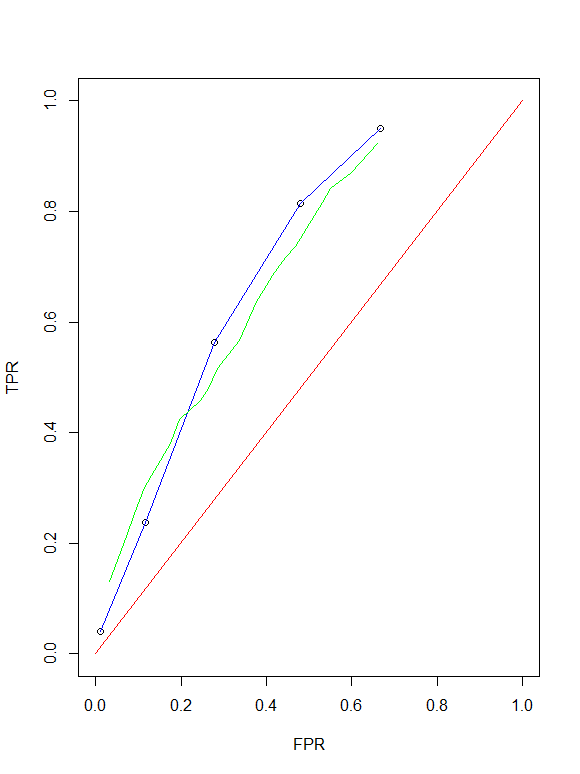
\includegraphics[width=\textwidth]{figures/Lab1_A1_ROC.png}  
  \caption{ROC - curve of  \textit{knearest} and  \textit{kknn}.\label{fig:ROC - curve} }
 \end{minipage}
\end{figure}
We see that out classifier, as observed in the confusion matrices, performs a couple of percentages better than \textit{kknn}.


\section{Assignment 2}

In this section the second assignment will be walked presented where the goal is to analyses a data set about the life length of a set of machines. The first part involves estimating the distribution and calculating the \textit{maximum logarithmic likelihood} for a machine to break down. 

We start by assuming the distribution 
\begin{equation}
  \mathbf{D} = \theta * e^{-\theta * \mathbf{X}}
\end{equation}
where \(\mathbf{x}\) is the observed life time of a set of machines and \( \mathbf{D} \) is the resulting vector ob observations. We will be trying out different values of \(\theta\). For this analysis we will try the range \( \theta = 0.1,...,100\) in  \(1\):s increments. The result can be observed in the plot below.
\begin{figure}[H]
\centering
\begin{minipage}[]{0.5\textwidth}
  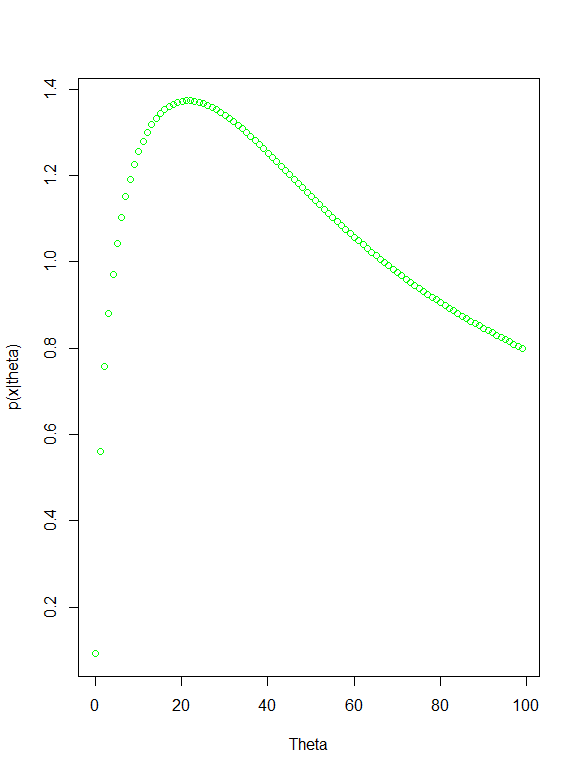
\includegraphics[width=\textwidth]{figures/Lab1_A2_data_distribution.png}  
  \caption{Distribution of the data set \textit{machines}.\label{fig:Distribution of the data set machines} }
 \end{minipage}
\end{figure}
The distribution seems to follow a typical exponential distribution where each observation is independent (as already specified for the data set). This can also be refered to as a \textit{Poisson distribution}.

We then try to find the log-likelihood \(log(p(\textbf{b} | \theta))\) using the result of above analysis. This is done by \( log( \mathbf{D} )\) for all \(\theta\) in the range \(0.1,...,20\) with \(0.1\) increments. multiple observations for each \( \theta \) we use the formula 
\begin{equation}
  log( \prod p(\mathbf{x} |\theta))
\end{equation}
where we do the \( \prod \) over all observations for a given \(\theta\) this is equivalent with the formula
\begin{equation}
  \sum{log(p(\mathbf{x} |\theta))}
\end{equation}
The result is plotted below, both for the full data set (red) and for the first six observations (green).
\begin{figure}[H]
\centering
\begin{minipage}[]{0.5\textwidth}
  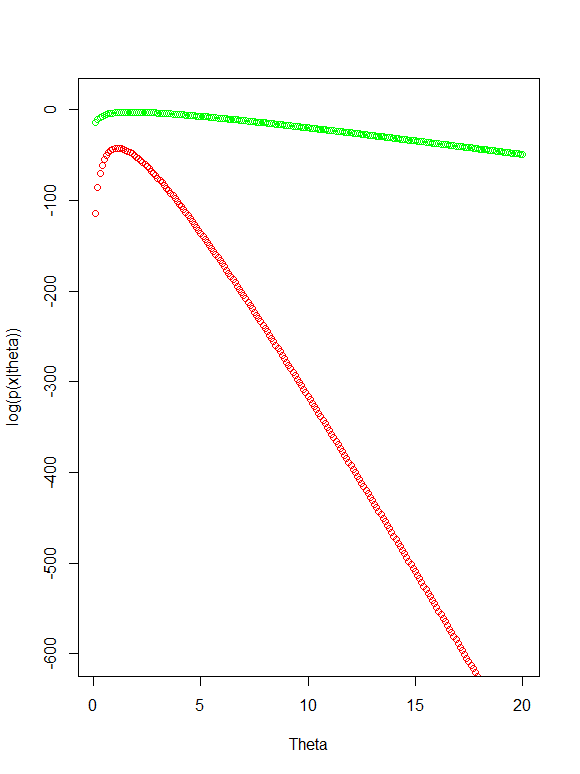
\includegraphics[width=\textwidth]{figures/Lab1_A2_ll_and_ll6.png}  
  \caption{Maximum log-likelihood for the full data set and the first 6 observations.\label{fig:Maximum log-likelihood for the full data set and the first 6 observations} }
 \end{minipage}
\end{figure}
The main takeaway from this plot is that 6 observations are not enough to perform a reliable likelihood estimation and that the theta resulting in the highest likelihood is \(\theta = 1.1\).

The next task is to calculate the posterior probabilities using the \textit{Bayesian model}: 
\begin{equation}
  p(x|\theta) = \theta * e^{-\theta * \mathbf{x}}
\end{equation}
and prior probability \(p(\theta) = \lambda * e^{-\lambda*\theta} \) with \( \lambda = 10\).  

To calculate this we create the function \(I(\theta) = log(p(\textbf{x}|\theta) * p(\theta))\).  The resulting ''curve'' can be observed bellow.
\begin{figure}[H]
\centering
\begin{minipage}[]{0.5\textwidth}
  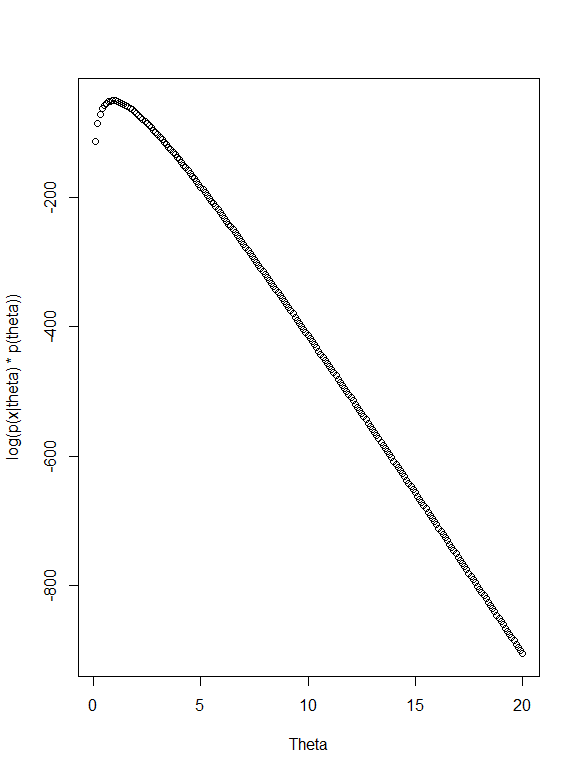
\includegraphics[width=\textwidth]{figures/Lab1_A2_post.png}  
  \caption{Posteriori likelihood of the data set \textit{machines}.\label{fig:Postpriori likelihood of the data set machines} }
 \end{minipage}
\end{figure}
Although \( log(p(\mathbf{x}))\) follows a exponential decrease curve the \(p(\theta)\) follows a linear curve and is huge compared to \( log(p(\mathbf{x}))\). The maximum \(\theta\) has gone from \(1.1\) to \(0.9\).

The final step involves generating 50 new observations from the exponential distribution by using the \(\theta = 1.1\). These observations will then be ploted in a histogram and compared to a histogram of the machine lifetime data set.

\begin{figure}[H]
\centering
\begin{minipage}[]{0.4\textwidth}
  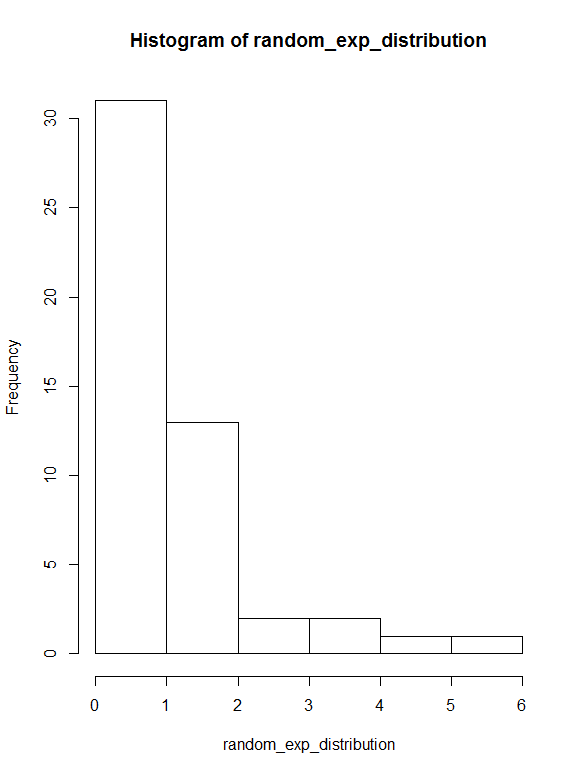
\includegraphics[width=\textwidth]{figures/Lab1_A2_hist_exp.png}  
  \caption{Histogram over 50 random samples from exponential distribution.\label{fig:Histogram over 50 random samples from exponential distribution} }
 \end{minipage}
\begin{minipage}[]{0.4\textwidth}
  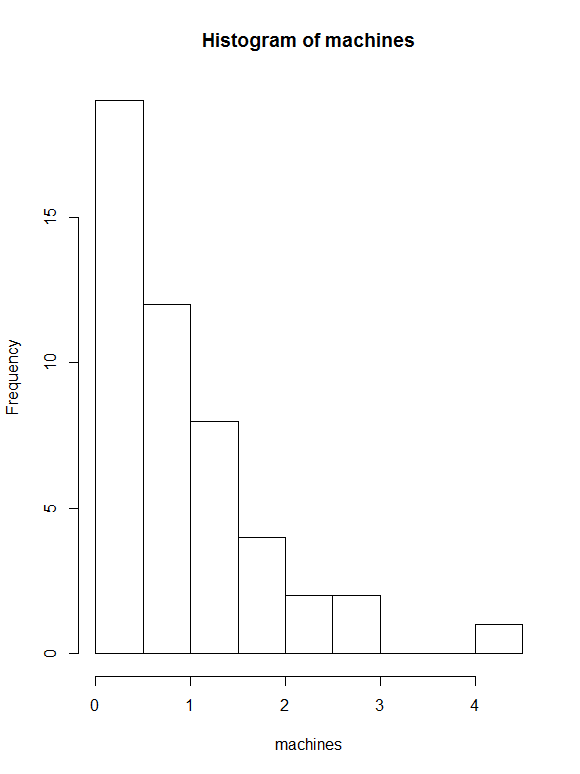
\includegraphics[width=\textwidth]{figures/Lab1_A2_hist_machines.png}  
  \caption{Histogram over the data set \textit{machines}.\label{fig:Histogram over the data set machines} }
 \end{minipage}
\end{figure}
The scale of the values in the two histograms differs greatly but the overall distribution of the values are very similar. If further proof of the \textit{machines} data set was distributed in a exponential fashion was needed it can be observed here.

\section{Appendix: A - Code assignment 1}

\lstinputlisting[caption=Code for assignment 1,
    label={assignment1.r},
    breaklines=true]
    {code/assignment1.r}

\section{Appendix: B - Code assignment 2}

\lstinputlisting[caption=Code for assignment2 ,
    label={assignment2.r},
    breaklines=true]
    {code/assignment2.r}
\end{document}
